\section{Bestiaire}

\subsection{Rakghoul}
\label{sec:rakghoul}
\noindent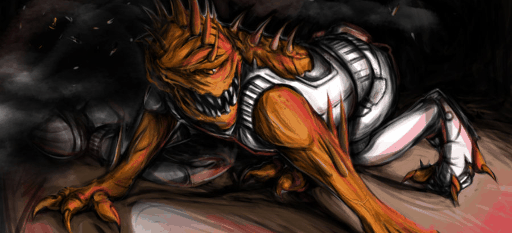
\includegraphics[width=\linewidth]{_img/dos-au-muur/rakghoul.png}

\subsubsection{Traits}

\begin{itemtable}[ c c c c c ]
    \textbf{Agi} & \textbf{Int} & \textbf{\^Ame} & \textbf{For} & \textbf{Vig} \\
    d8           & d6           & d6             & d8           & d8
\end{itemtable}
\begin{itemtable}[ l X ]
    \textbf{Allure}      & 6 \\
    ~                    & Vision Nocturne \\
    ~                    & Marche sur les murs \\
    \textbf{Compétences} & Combat d8, Discrétion d6
\end{itemtable}

\subsubsection{Défense}
\begin{itemtable}[ c c ]
    \textbf{Parade}     & \textbf{Résistance} \\
    6                   & 6 
\end{itemtable}

\subsubsection{Attaque}
\begin{itemtable}[ X c c ]
    ~       & \textbf{Combat}   & \textbf{Dégats} \\
    Griffes & d8                & 1d6 
\end{itemtable}

\newpage
\subsubsection{Background}
Les Rakghouls sont une espèce issue d’une maladie créée par le seigneur Sith Karness Muur. Les individus atteint par cette maladie deviennent des monstres incapables de penser par eux-mêmes. Karness peut les contrôler grâce à son talisman (Le Talisman de Muur).

La maladie se transmet par une griffure ou une morsure mais cela ne fonctionne pas avec les êtres sensibles à la Force. Karness a créé ce virus à partir du coté Obscur de la Force ce qui explique une forte présence obscure près de ces monstres.

Karness a créé plusieurs versions du virus car les premiers Rakghouls ne répondaient pas bien au contrôle de Karness. Les nouveaux sont plus réceptifs et plus fort.

Quand le Talisman de Muur a été perdu dans les bas fonds de Taris, on a peu constaté que les créatures, suite à une exposition prologée au Talisman finissaient par se transformer en Rakghouls. Mais les Rakghouls transformé de cette façon sont bestiaux, stupides et sans âme. Ils attaquent tout ce qui bouge. Ces créatures ne fonctionnent qu’à l’instinct.

\clearpage
\subsection{Rakghoul Amblyope}
\label{sec:rakghoul-amblyope}
\noindent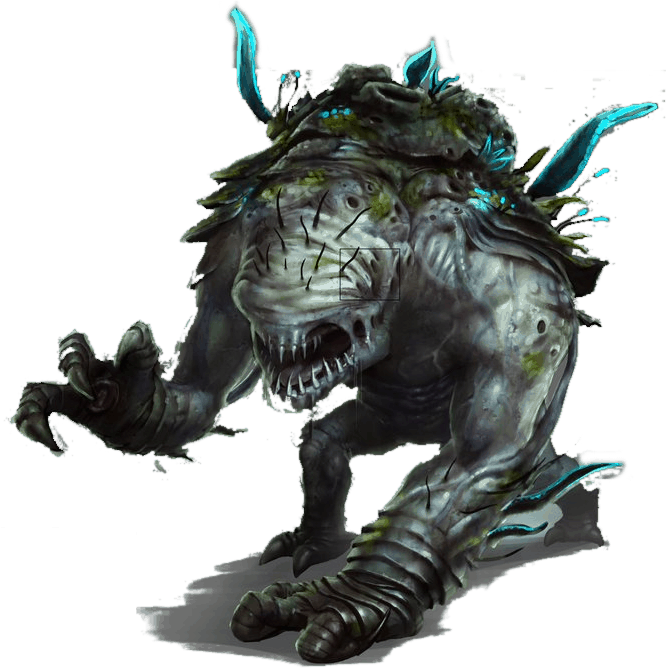
\includegraphics[width=\linewidth]{_img/dos-au-muur/rakghoul-amblyope.png}

\subsubsection{Traits}

\begin{itemtable}[ c c c c c ]
    \textbf{Agi} & \textbf{Int} & \textbf{\^Ame} & \textbf{For} & \textbf{Vig} \\
    d4           & d6           & d6             & d12+2        & d10
\end{itemtable}
\begin{itemtable}[ l X ]
    \textbf{Allure}      & 5 \\
    \textbf{Taille}      & +5 \\
    ~                    & Vision de Force \\
    ~                    & \'Enorme (+2 pour les jets d’attaque adverses)\\
    \textbf{Compétences} & Combat d10
\end{itemtable}

\subsubsection{Défense}
\begin{itemtable}[ c c ]
    \textbf{Parade}     & \textbf{Résistance} \\
    5                   & 12 
\end{itemtable}

\subsubsection{Attaque}
\begin{itemtable}[ X c c ]
    ~           & \textbf{Combat}   & \textbf{Dégats} \\
    Mains nues  & d10               & d12+2 
\end{itemtable}

\newpage
\subsubsection{Background}
Version stéroïdée des Rakghouls standard, Amblyope est notre petit boss de niveau.

Quand les Rakghouls sont livrés à eux-mêmes et qu’ils laissent libre cours à leurs plus bas instincts, il arrive qu’un Rakghoul plus fort que les autres s’en prenne à ces petits camarades et les dévore sans scrupules. Cet afflux de Force Obscure peut le faire muter et le Rakghoul devient une espèce de gros monstre de 3m de haut, complètement aveugle mais attiré par les émanations de Force, il attaque machinalement les adversaires les plus sensibles à la Force. 

\clearpage
\subsection{Vyna Anen} \label{sec:vyna-anen}
\noindent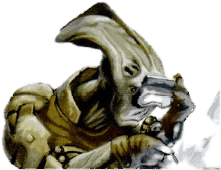
\includegraphics[width=\linewidth]{_img/dos-au-muur/vyna-anen.png}

\textbf{Race:} Sluissi

\subsubsection{Traits}

\begin{itemtable}[ c c c c c ]
    \textbf{Agi} & \textbf{Int} & \textbf{\^Ame} & \textbf{For} & \textbf{Vig} \\
    d6           & d10          & d6             & d4           & d6
\end{itemtable}
\begin{itemtable}[ l X ]
    \textbf{Allure}      & 6 \\
    \textbf{Compétences} & Intimidation d6, Persuasion d12, Réseaux d6
\end{itemtable}

\subsubsection{Défense}
\begin{itemtable}[ c c ]
    \textbf{Parade}     & \textbf{Résistance} \\
    2                   & 5 
\end{itemtable}

\newpage
\subsubsection{Background}
\noindent
\includegraphics[width=\linewidth]{_img/dos-au-muur/industrial-automaton.png}

Vyna Anen est l’un des agents de liaison entre Industrial Automaton et l’Empire. Officiellement employé par IA comme secrétaire au service des "Projets Spéciaux". 

Vyna est un homme pragmatique qui fait ce que l’Empire lui demande sans poser de questions, sans scrupules ni états d’âme. C’est un fin négociateur entièrement voué à l’Empire.\\

\subsection{Garan Keggle}  \label{sec:garan-keggle}